% !TeX root = ./tesi.tex
% !TeX encoding = UTF-8 Unicode
% !TeX spellcheck = it_IT
% !TeX program = arara
% !TeX options = --log --verbose --language=it "%DOC%"

% arara: lualatex:      { interaction: batchmode }
% arara: frontespizio:  { interaction: batchmode, engine: lualatex }
% arara: biber
% arara: lualatex:      { interaction: batchmode }
% arara: lualatex:      { interaction: nonstopmode, synctex: yes }

\documentclass[%
  a4paper,                % formato di pagina A4
  12pt,                   % corpo del testo a 12pt
  % la dimensione 12pt automaticamente imposta \footnotesize a 10pt
  twoside,                % (oneside|twoside) documento a singola o doppia facciata,
  openright,              % (openany|openright) fa cominciare un capitolo nella successiva pagina a disposizione o sempre in una pagina destra
  % twocolumn,            % dà a LaTeX le istruzioni per comporre l'intero documento su due colonne
  titlepage,              % (titlepage|notitlepage) se dopo il titolo del documento debbaavere  inizio  una  nuova  pagina
  % fleqn,                % allinea le formule a sinistra rispetto a un margine rientrato
  % leqno,                % mette la numerazione delle formule a sinistra anziché a destra
  final                   % (draft|final) scelta tra bozza o finale, influenza il comportamento degli altri pacchetti
]{scrbook}

\usepackage{fancyvrb}       % fornisce l'ambiente VerbatimOut e modifica listati di codice
% \usepackage{minted}       % evidenzia la sintassi dei listati di codice; richiede pygments installato e shell-escape

\begin{VerbatimOut}{\jobname.xmpdata}
\Title{Titolo}
\Subject{Oggetto}
\Author{Niccolò Maltoni}
\Copyright{Questo documento è fornito sotto licenza Apache License, Version 2.0}
\CopyrightURL{https://opensource.org/licenses/Apache-2.0}
\end{VerbatimOut}

\usepackage[%
  english,italian             % definizione delle lingue da usare
]{varioref}                     % introduce il comando \vref da usarsi nello stesso modo del comune \ref per i riferimenti

\usepackage[a-1b]{pdfx}

%% Font
% non è necessario \usepackage[utf8]{inputenc} perché luaLaTeX accetta solo UTF-8
\usepackage{fontspec}
\setmainfont[%
  Ligatures=TeX               % abilita legature classiche di LaTeX
]{Latin Modern Roman}           % imposta il font con grazie per il testo principale
\setsansfont[%
  Ligatures=TeX               % abilita legature classiche di LaTeX
]{Latin Modern Sans}            % imposta il font senza grazie
\setmonofont[%
  Ligatures=TeX               % abilita legature classiche di LaTeX
]{Latin Modern Mono}            % imposta il font teletype monospaziato

%% Matematica
\usepackage{amsmath}
% non bisogna assolutamente invocare il pacchetto amssymb
\usepackage[%
  math-style=ISO              % per scrivere la matematica delle scienze sperimentali bisogna seguire le norme ISO
]{unicode-math}                 % implementazione di glifi Unicode per caratteri matematici
\setmathfont[%
  Ligatures=TeX               % abilita legature classiche di LaTeX
]{Latin Modern Math}
\usepackage[%
  output-decimal-marker={,},  % le convenzioni tipografiche italiane prevedono la virgola e non il punto
  binary-units                % abilita le espressioni per bit e byte
]{siunitx}                      % permette di definire numeri con unità di misura

%% Lingue
\usepackage[%
  strict=true,                % converte tutti i warning in errori
  autostyle=true,             % adatta continuamente lo stile delle virgolette alla lingua
  english=american,           % imposta lo stile per l'inglese
  italian=guillemets          % imposta lo stile per l'italiano
]{csquotes}                     % configura le virgolette secondo gli stnadard della lingua
\usepackage{polyglossia}
\setmainlanguage[%
  babelshorthands             % attiva il carattere " come switch per virgolettature etimologiche
]{italian}                      % imposta l'italiano come lingua principale
\setotherlanguage[%
  variant=american            % imposta la variante americana dell'inglese
]{english}                      % imposta l'inglese come lingua secondaria
% non è necessario \usepackage{indentfirst} perché con lualatex il rientro del primo capoverso è preimpostato

%% Altri pacchetti
\usepackage{graphicx}           % serve per includere immagini e grafici
\graphicspath{{res/fig}}      % importa la cartella res/fig/ come cartella da cui caricare le immagini
\usepackage{xcolor}             % permette di usare colori
% \usepackage{subcaption}       % serve per ottenere sottofigure
% \usepackage{caption}          % permette di controllare la formattazione delle didascalie
% \usepackage{adjustbox}        % permette di effettuare il crop delle immagini
% \usepackage{ctable}           % permette di migliorare la spaziatura dell'ambiente tabular standard
% \usepackage{flafter}          % impedisce alle figure di apparire prima della loro definizione nel testo
\usepackage{scrhack}            % risolve incompatibilità tra KOMA e pacchatti vari (float, listings, ...)
\usepackage{float}              % permette di forzare il posizionamento dell’oggetto nel punto in cui è situato con l’opzione H
\usepackage{afterpage}          % permette di eseguire qualcosa nella pagina successiva con \afterpage{...} (ad esempio, figure)
% \usepackage{placeins}         % permette di mettere delle barriere invalicabili per le figure con \FloatBarrier
\usepackage[%
  write,                      % (write|nowrite) genera o meno il file
  standard,                   % (standard|suftesi) specifica tipo di frontespizio
  normal,                     % (normal|sans) usa font con grazie anziché senza
  noinputenc,                 % non carica inputenc (poiché usa lualatex)
  % norules,                  % non vengono inseriti filetti nel frontespizio
  nouppercase,                % con questa opzione verrà rispettato il maiuscolo e il minuscolo
  driver=luatex               % imposta la chiamata di graphicx nel documento frn per l'uso di un driver diverso da dvips o pdftex
]{frontespizio}
\usepackage{geometry}           % permettte la modifica della gabbia del documento
\geometry{
  a4paper,                    % formato di pagina
  heightrounded,              % modifica di poco le dimensioni della gabbia per contenere un numero intero di righe
  hmargin=2.5cm,              % dimensioni margini destro-sinistro
  vmargin=2.5cm               % dimensioni margini superiore-inferiore
}
\usepackage{setspace}           % serve a fornire comandi di interlinea standard
\onehalfspacing{}             % imposta interlinea a 1,5 ed equivale a \linespread{1,5}

%% Definizioni di comandi e ambienti
%% Definisco un nuovo comando per enfatizzare il testo in inglese %%%%%%%%%%%
\newcommand{\engEmph}[1] {\emph{\foreignlanguage{english}#1}}

%% Aggiunge pagine bianche vuote %%%%%%%%%%%%%%%%%%%%%%%%%%%%%%%%%%%%%%%%%%%%
\newcommand{\clearemptydoublepage}{\newpage{\pagestyle{empty}%
%\cleardoublepage}}
\clearpage}}

%% Definisce l'environment abstract per la classe book %%%%%%%%%%%%%%%%%%%%%%
\newenvironment{abstract}%
  {\cleardoublepage%
    \thispagestyle{empty}%
    \null\vfill\begin{center}%
      \bfseries\abstractname\end{center}}%
  {\vfill\null}

\usepackage[%
  maxcitenames=2,             % massimo numero di nomi nelle citazioni
  mincitenames=2,             % minimo numero di nomi nelle citazioni
  maxbibnames=99,             % massimo numero di nomi nella blibliografia
  minbibnames=99,             % minimo numero di nomi nella blibliografia
  style=ieee,                 % imposta lo stile della blibliografia (numeric|alphabetic|authoryear|authortitle|verbose|...)
  giveninits=true,
  backend=biber               % specifica il backend per la bibliografia
]{biblatex}                     % si interfaccia con bibtex e biber per la bibliografia
\addbibresource{biblio.bib}
\usepackage[%
  % page,                     % Aggiunge una pagina con la scritta Appendices
  % toc,                      % Aggiunge un campo Appendices nell'indice
  titletoc,                   % Aggiunge la parola Appendice per ogni capitolo dell'appendice nell'indice
  title%                      % Aggiunge la parola Appendice per ogni capitolo dell'appendice
]{appendix}                     % modifica la gestione dell'appendice, e aggiunge l'ambiente appendices alternativo al comando \appendix
% \usepackage[htt]{hyphenat}    % permette la sillabazione dei blocchi di testo monospaziato
% \usepackage{enumerate}        % aggiunge un argomento opzionale che determina come comporre l’etichetta numerata delle liste

\usepackage{microtype}          % gestisce la microtipografia

% \usepackage{hyperref}         % gestisce tutte le cose ipertestuali del pdf; importato automaticamente
\hypersetup{%
  pdfpagemode={UseNone},
  hidelinks,                  % nasconde i collegamenti (non vengono quadrettati)
  hypertexnames=false,
  linktoc=all,                % inserisce i link nell'indice
  unicode=true,               % usa solo caratteri Latini nei segnalibri di Acrobat
  pdftoolbar=false,           % nasconde la toolbar di Acrobat
  pdfmenubar=false,           % nasconde il menu di Acrobat
  plainpages=false,
  breaklinks,
  pdfstartview={Fit},
  pdflang={it}
}

\usepackage[%
  english,italian,            % definizione delle lingue da usare
  nameinlink                  % inserisce i link nei riferimenti
]{cleveref}                     % permette di usare riferimenti migliori dei \ref e dei varioref

\begin{document}

  \frontmatter{}
  \pagenumbering{Roman}
  \pagestyle{empty}
  % !TeX root = ../../tesi.tex
% !TeX encoding = UTF-8 Unicode
% !TeX spellcheck = it_IT

\begin{Preambolo*}
  \usepackage{fontspec}
  \setmainfont[Ligatures=TeX]{Latin Modern Roman}
\end{Preambolo*}
\begin{frontespizio}
  \Universita{Bologna}        % aggiunge da sé “Università degli Studi di”.
  \Istituzione{%
    Alma Mater Studiorum --- Università di Bologna \\%
    Campus di Cesena%
  }
  \Divisione{Dipartimento di Informatica --- Scienza e Ingegneria}
  \Corso[Laurea magistrale]{Ingegneria e Scienze Informatiche}
  \Annoaccademico{2019--2020}
  \Titolo{Clustering di traiettorie in ambito Big Data}
  \Sottotitolo{Tesi in Data Mining}
  % \Preambolo{\renewcommand{\frontsmallfont}[1]{\small}}       % non viene stampata la matricola
  % \Preambolo{\renewcommand{\frontsmallfont}[1]{\small Matr.}} % abbrevia la matricola
  \Candidato[0000852918]{Federico~Naldini}
  \NCandidato{Presentata da}  % sostituisce la parola “Candidato”
  \Relatore{Prof.~Matteo~Golfarelli}
  \Correlatore{Dott.~Matteo~Francia}
  \Piede{%                    % sostituisce la scritta “Anno Accademico” nel piede
    III sessione di laurea \\%
    Anno Accademico 2019--2020%
  }
\end{frontespizio}

  % !TeX root = ../../tesi.tex
% !TeX encoding = UTF-8 Unicode
% !TeX spellcheck = it_IT

\clearemptydoublepage{}
\thispagestyle{empty}
\vspace*{20ex}
\begin{flushright}
    \begin{LARGE}
        \textbf{Parole chiave}\\
        \vspace{5ex}
    \end{LARGE}
    \begin{normalsize}
        \textbf{%
            Trajectory mining\\%
            \medskip
            Trajectory clustering\\%
            \medskip
            Big data%
        }
    \end{normalsize}
\end{flushright}
\vfill

  % !TeX root = ../../tesi.tex
% !TeX encoding = UTF-8 Unicode
% !TeX spellcheck = it_IT

\clearemptydoublepage{}
\null{}\vspace{\stretch{1}}
\begin{flushright}
    \textit{Dedica}
\end{flushright}
\vspace{\stretch{2}}\null{}

  % !TeX root = ../../tesi.tex
% !TeX encoding = UTF-8 Unicode
% !TeX spellcheck = it_IT

\begin{abstract}
  Abstract
\end{abstract}

  \tableofcontents

  \mainmatter{}
  \pagenumbering{arabic}
  \pagestyle{headings}
  \chapter{Clustering di traiettorie}\label{chapter:chapter1}
  
\section{Problematica}\label{sec:problem}
Uno degli obiettivi dell'analisi di dati di traiettoria è il \textit{clustering} (raggruppamento) di traiettorie simili.
Una traiettoria può essere considerata non solo come il tragitto percorso dall'oggetto che la genera,
ma anche come l'insieme delle attività, ciascuna corrispondente a una posizione, eseguite dal medesimo oggetto.
Lo scopo del clustering di traiettorie è quindi di scoprire quali condividono una certa similarità e quali invece no.
In tal modo è possibile identificare eventuali raggruppamenti di oggetti che hanno percorso assieme una certa frazione del loro percorso, oppure individuare eventuali
traiettorie differenti da tutte le altre.
Interpretando poi questi risultati partendo dalle traiettorie come insiemi di attività, è possibile ad esempio dedurre quali possano essere attività comuni e quali invece no.


\subsection{Clustering}\label{subsec:problem:clustering}
Il clustering, o analisi di raggruppamento, è una tecnica non supervisionata con lo scopo di aggregare i dati in \textit{cluster} o gruppi
tali che i dati all'interno di un gruppo siano più simili tra loro rispetto a quelli all'esterno\cite{liao2005clustering, zazzarro2009clustering}.

I metodi di clustering per elaborare dati statici di differenti tipologie sono cinque:

\begin{itemize}
  \item Metodi basati sul partizionamento:
  \item Metodi basati sulla gerarchia:
  \item Metodi basati sulla densità:
  \item Metdi basati su una griglia:
  \item metodi basati sul modello:
\end{itemize}




\subsection{Dati di traiettoria}\label{subsec:problem:trajectorydata}
Negli ultimi anni, la grande presenza di dipositivi in grado di catturare la posizione di un oggetto nel
tempo e le sue variazioni hanno prodotto enormi quantità di dati.
L'analisi di questi dati, resa possibile dalle moderne tecnologie Big Data, apre molteplici possibilità, come
ad esempio la ricerca dei flussi di traffico all'interno di un terriorio cittadino, oppure l'individuazione
dei luoghi più visitati da una certa categoria di utenti, o ancora il riconoscimento di gruppi di oggetti che si
muovono assieme all'interno di un certo spazio e tempo.
Dato il grande numero di potenziali fonti per i dati, è necessario ricondurre questi ultimi a una formulazione comune
così da poter sfruttare al meglio le loro potenzialità espressive.
La rappresentazione più basilare consiste nel considerare una traiettoria come l'insieme delle posizioni
spaziali dei punti che la compongono associando a ciascuno l'istante temporale in cui è stato registrato.
Questa formulazione prende il nome di traiettoria grezza (\textit{raw trajectory}), vedi~\cref{fig:chap-1:trajectory}
Andando a formalizzare quanto detto sopra:

\begin{figure}
  \centering
  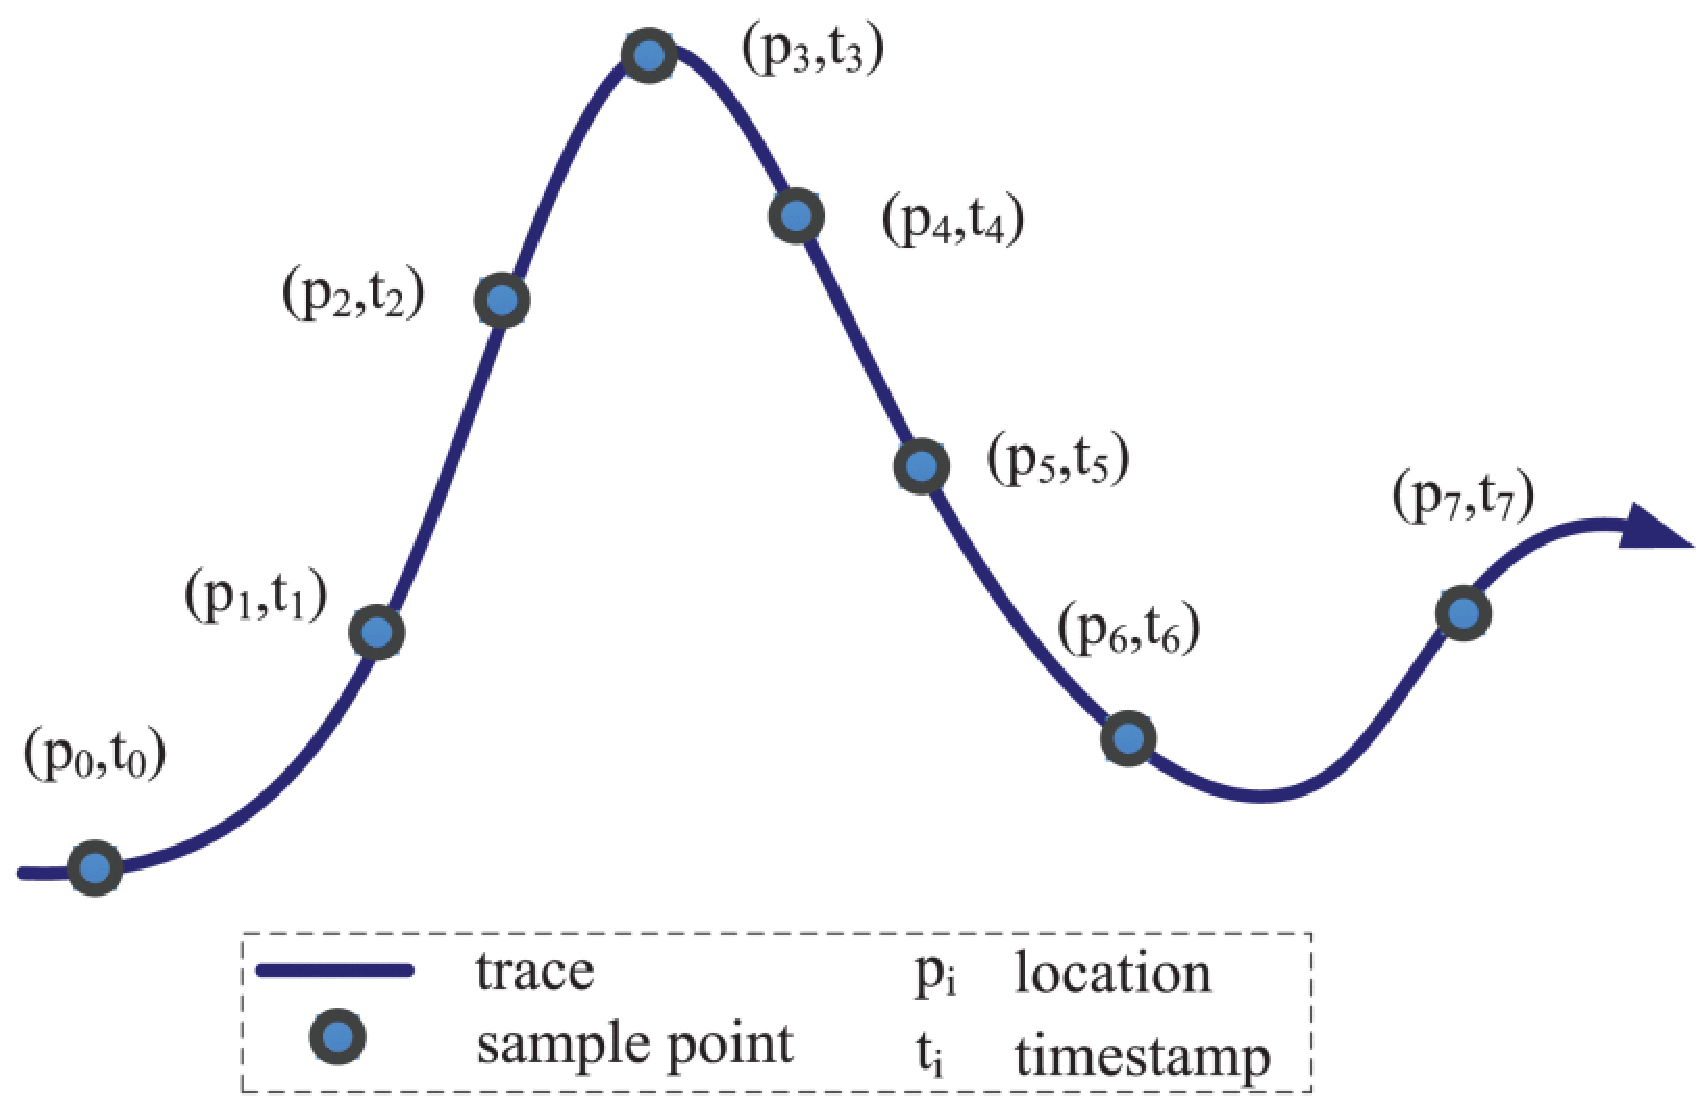
\includegraphics[scale=.5]{/sec-1/trajectory.pdf}
  \caption{Esempio di traiettoria,Fonte:\url{https://www.semanticscholar.org/paper/A-Survey-on-Trajectory-Data-Mining\%3A-Techniques-and-Feng-Zhu/a32f521442a540a6d1420526eaa68b3cab6b1d0d}}%
  \label{fig:chap-1:trajectory}
\end{figure}

\begin{definition}[Traiettoria]

  Si definisce una traiettoria grezza, o \textit{raw trajectory}, una sequenza temporale di punti \({p_{t}, p_{t'},\ldots, p_{t''}}\)
  tale che ogni punto \(p_{t}\) è composto da una coppia di coordinate spaziali \((latitude, longitude)\) e un tempo~\(t\).

\end{definition}

Questa basilare e semplice modalità di espressione può essere successivamente complicata, ad esempio adottando
una scala unica tra le diverse traiettorie per lo spazio e una per il tempo, oppure aggiungendo ulteriori informazioni, come ad esempio la direzione o attributi
dell'oggetto che la genera.

Per aumentare l'espressività della singola traiettoria, può essere utile definire il concetto di sotto-traiettoria, o \textit{subtrajectory}.
Intuitivamente una sotto-traiettoria non è altro che un segmento di una traiettoria relativo a un certo sottoinsieme dello spaziotempo coperto da quest'ultima.

\begin{definition}[Sottotraiettoria]

  Date due traiettorie \(TR\textsubscript{i}, TR\textsubscript{j}\) si definisce  \(TR\textsubscript{i}\) sottotraiettoria di \(TR\textsubscript{j}\) se \(\forall p_{t\textsubscript{i}} \in TR\textsubscript{i}, p_{t\textsubscript{i}} \in TR\textsubscript{j}\).

\end{definition}

Una volta definito che cos'è un dato di traiettoria, occorre mettere in chiaro che cosa distingue una traiettoria da un'altra.
Prendendo ad esempio il problema del clustering, sarebbe sbagliato tentare di applicare le stesse metriche di similarità anche ai dati di traiettoria
poiché gli oggetti in movimento producono spesso dati ad alta dimensionalità e con particolari correlazioni tra le dimensioni.
Il problema risulta quindi decisamente articolato: uno buona metrica di similarità deve tenere conto non solo dei singoli punti, ma anche della
traiettoria nella sua interezza, considerando anche la diversa lunghezza tra i due soggetti del confronto.
In letteratura sono presenti diversi metriche che possono essere impiegate nel confronto tra traiettorie:

\begin{itemize}

  \item \textbf{Distanza Euclidea.}
  La più semplice tra tutte le misure di stanza presentate, grazie alla sua complessità lineare permette di gestire dati ad alta dimensionalità.
  Date due traiettorie  \(T\textsubscript{i}\) e  \(T\textsubscript{j}\) di lunghezza \(n\) e dimensioni \(p\), la loro distanza euclidea si definisce come:

  \begin{equation}
    {D_E(T_{i}, T_{j}) = { {\frac{1}{n} } \sum_{k=1}^{n} {\sqrt{\sum_{m=1}^{p}{(a_{k}^{m} - b_{k}^{m})}^2}}}}
  \end{equation}

  La metrica tuttavia non è esente da difetti: è molto sensibile al rumore e richiede che le traiettorie siano uguali per numero di punti
  e dimensioni, inoltre anche l'intervallo di campionamento temporale deve coincidere. Questi limiti sono abbastanza difficili da
  aggirare quando si processa un dataset reale.

  Per superare questi problemi, sono disponibili diverse varianti della distanza euclidea: una su tutte è la \textit{Principal Component Analysis Plus Euclidean Distance} (PCA + distance)~\cite{zhang2006comparison}.
  Questa tecnica prima riduce le dimensioni spaziali ad una sola, successivamente esegue un'analisi PCA per convertire ogni traiettoria in
  \textit{k} coefficenti; a questo punto viene calcolata la distanza euclidea considerando i valori dei coefficenti individuati dall'analisi.
  Questa variazione mantiene gli stessi punti di forza della versione base della metrica, in più consente una maggior resistenza al rumore.



  \item \textbf{Distanza di Hausdorff.}
  La distanza di Hausdorff~\cite{chen2011clustering} misura quanto due traiettorie sono distanti l'una dall'altra.
  Date due traiettorie, per ogni punto di una viene calcolato il più vicino punto dell'altra e la distanza tra i due, il valore della distanza di Hausdorff
  corrisponde alla massima distanza calcolata nel passo precedente.~\cref{def:Hausdorff}
  \begin{equation} \label{def:Hausdorff}
    {D_{Hausdorff}(T_{i}, T_{j}) = \max{(h(T_{i}, T_{j}), h(T_{j}, T_{i}))}}~where~{h(T_{i}, T_{j}) = \max_{a \in T_{i}}{(\min_{b \in T_{j}}{(dist(a,b))})}}
  \end{equation}

  Nella formula \(h\) rappresenta la distanza di Hausdorff diretta, mentre \(d\) la distanza euclidea tra due punti.
  Il calcolo di entrambe le distanze dirette permette di gestire traiettorie con numero di punti differente tra loro.
  Questa metrica risulta robusta rispetto all'influenza causata da particolari distribuzioni di punti, ma allo stesso tempo è sensibile
  al rumore. Dalla formula~\cref{def:Hausdorff} è possibile definire la complessità computazionale della metrivca come \(O(m*n)\).


  \item \textbf{Distanza LCSS.}
  Longest Common Sub Sequence~\cite{rick2000efficient} affronta il problema con un approccio diverso: invece che calcolare la distanza fra i punti tra le due traiettorie, computa la
  più lunga sotto-sequenza.
  La lunghezza di quest'ultima determina la vicinanza,: più il valore è alto più le due traiettorie sono vicine.
  Essendo impossibile una coincidenza assoluta dei punti tra due traiettorie sono definite due soglie, \(\epsilon \) e \( \sigma \) che rispettivamente
  modellano la tolleranza rispetton all'asse x e y.
  LCSS può essere calcolata in modo ricorsivo, il suo tempo di computazione coincide con la diatnza di Hausdorff, inoltre consente una certa tolleranza rispetto
  alle deviazioni nei dati, ciò consente una buona efficenza nei dataset reali. Il maggior limite della metrica sta nella definizione dei parametri
  \(\epsilon \) e \( \sigma \) in problemi complessi.

  \item \textbf{Distnza DTW.}
  Dynamic time warping (DWT)~\cite{chen2005robust} pone il focus sulla dimensione temporale rispetto a quelle spaziali, come accadeva nelle metriche precedenti.
  Lo scopo è trovare l'allineamento ottimo tra due traiettorie dati certi vincoli.
  DWT resiste bene alle differenti lunghezze tra traiettorie: obbiettivo della misura è infatti ricercare il percorso a cui assimilare le traiettorie che abbia il minor coeficcente di distorsione,
  calcolato sulle trasformazioni subite dalle traiettorie.
  DWT assicura il rispetto dell'ordine tra i punti delle traiettorie, inoltre introducendo un principio di scaling locale della dimensione temporale,
  riesce a gestire scale temporali differenti tra le traiettorie.
  Tuttavia richiede continuità all'interno dei punti, è sensibile al rumore e a sottotraiettorie molto distanti tra loro.
  La complessità di questa misura è \(O(m*n)\).


  \item \textbf{Distanza di Fréchet.}
  La metrica di Fréchet~\cite{khoshaein2013trajectory} considera in contemporanea sia la dimensione temporale
  che quella spaziale durante il calcolo della distanza.
  Date due traiettorie di uguale lunghezza \(n\), si calcola la distanza euclidea tra i punti aventi stessa posizione all'interno delle due traiettorie:
  il valore più alto corrisponde alla distanza di Fréchet.
  Qualora le due traiettorie divergano come dimensioni, si eseguirà questo calcolo su tutte le possibili sotto-traiettorie di lunghezza \(n\) generabili
  dalla traiettoria più lunga.
  La complessità della misura nel caso peggiore è \(O(m*n)\).
  La distanza di Fréchet considera la traiettoria nella sua continuità, per questo motivo è molto sensibile agli outlier.


\end{itemize}





\section{Clustering di dati di traiettoria}\label{sec:problem:trajectoryclustering}

Come detto nella~\cref{sec:measure}, i dati di traiettoria sono molto più complessi
rispetto ai dati solitamente utilizzati con gli algoritmi di clustering tradizionali.
Occorre quindi definire modifiche di questi ultimi per riuscire a fare operazioni di clustering
efficienti, in quanto sarebbe impossibile catturare tutta la complessità dell'informazione con
tecniche pensate per dati a bassa dimensionalità.

Alla luce di quanto detto sopra, per il clustering di traiettorie sono individuabili i seguenti obbiettivi:

\begin{itemize}

  \item \textbf{Supporto alla dimensionalità dei dati}.
  Obbiettivo del clustering di traiettorie è la ricerca di cluster tenendo conto di tutte le informazioni presenti sui dati.
  Ognuno di questi attributi dovrà essere considerato nel momento in cui verranno portate avanti le operazioni di divisione e raggruppamento delle traiettorie.

  \item \textbf{Definizione di una metrica di similarità tra traiettorie}.
  Come presentato nella~\cref{sec:measure} il problema della similarità tra traiettorie è complesso e sono presenti diverse soluzioni.
  Scopo della ricerca è quello di individuare metriche che individuino le differenze tra le traiettorie in maniera affidabile e efficace.

  \item \textbf{Qualità dell'algoritmo}.
  L'algoritmo utilizzato nelle operazioni di clustering deve essere efficiente e scalabile, ad esempio impiegando apposite strutture dati per
  ridurre i tempi di accesso ai dati, oppure utilizzando le tecnologie di computazione Big Data per velocizzare l'esecuzione degli algoritmi.

\end{itemize}

Nonostante nessuno degli algoritmi di clustering tradizionali abbia tutte le caratteristiche espresse sopra, le idee alla loro base rimangono comunque
valide in buona parte dei casi.
Di conseguenza molti algoritmi pensati per i dati di traiettoria non sono che estensioni di quelli già noti in letteratura.

Gli algoritmi di clustering di traiettorie sono 
classificabili secondo la natura del dato in output
e sulla tipologia di clustering.
La natura del dato è direttamente collegata alle dimensioni considerate nelle operazioni di clustering:
la ricerca può essere condotta considerando solo la componente spaziale o includendo anche quella temporale.
La tipologia di clustering invece riguarda i cluster prodotti in output: algoritmi partizionanti 
produrranno cluster disgiunti, algoritmi di clustering sovrapposto cluster la cui intersezione non è vuota.

La \cref{tab:clus-alg} riassume i principali algoritmi che saranno trattati nelle sezioni successive alla luce della classificazione appena introdotta.
\begin{table}[H]
    \centering
   \begin{tabular}{||c c c||}
 \hline
 Algoritmo & Natura dei dati & Tipologia di clustering \\ [0.5ex] 
 \hline\hline
CB-SMoT & Spaziale & Sovrapposto \\ 
 \hline
CACT & Spaziale & Sovrapposto \\ 
 \hline
T-OPTICS & Spazio-temporale & Sovrapposto \\
 \hline
TraceMob & Spaziale & Partizionante \\
 \hline
 DSC & Spazio-temporale & Sovrapposto \\
 \hline

\end{tabular}
    \caption{Classificazione degli algoritmi di clustering di traiettorie trattati}
    \label{tab:clus-alg}
\end{table}

\begin{center}

\end{center}


\subsection{Algoritmi Spaziali}\label{subsec:problem:spatialalgorithms}
Le informazioni spaziali sono probabilmente la feature più importanti all'interno di un dato di traiettoria.
Analizzando come un oggetto si muove e i luoghi che visita possono essere ricavate una vasta serie di informazioni.
Negli anni vari algoritmi sono stati proposti per estrarre dai dati informazioni differenti tra loro.

Il primo ambito di ricerca sui dati spaziali riguarda i luoghi di maggior interesse, ovvero le posizioni
in cui sono passati un certo numero di oggetti all'interno del dataset.
A questa categoria appartiene il framework \textit{CB-SMoT} (Clustering Based Stop and Moves of Trajectories)~\cite{palma2008clustering}.
Questo algoritmo ricerca all'interno delle varie traiettorie considerando gli stop, ovvero segmenti in cui la velocità della traiettoria cala sotto una certa soglia o risulta uguale a zero.
Successivamente questi segmenti sono raggruppati in cluster usando una versione modificata di DBSCAN\@.
Tale versione dell'algoritmo si basa sulla velocità invece che sulla densità.
Infine ogni cluster viene confrontato con la mappa dell'area coperta dalle traiettorie e viene associato a uno specifico punto o area.
Questa associazione permette di interpretare meglio il risultato ottenuto dall'algoritmo.


Ancora è possibile estrarre da un insieme di dati di traiettorie, l'insieme delle strade più
frequentate; ciò diverge dal primo ambito presentato poiché la ricerca di un percorso risulta
più complessa rispetto a quella di un singolo punto: una strada infatti ha caratteristiche molto
più complesse di una singola località, come ad esempio una continuità nello spazio tra i vari punti che
la compongono.
\textit{CACT}~\cite{hung2015clustering} (Clustering and Aggregating Clues of Trajectories) è un possibile framework per
ricercare percorsi che rappresentino i comportamenti di una certa categoria di utenti.
L'idea dell'algoritmo è di definire una misura di similarità basata sugli indizi (\textit{clue}):
Un indizio è definibile come la vicinanza spazio-temporale di punti di traiettorie diverse che però condividono lo stesso comportamento.
Tale indizio costituisce una corrispondenza parziale di comportamento.
Sulla base della presenza di indizi simili, vengono costituiti cluster di traiettorie, che raggruppano queste ultime sulla base di un certo comportamento.
I cluster così ottenuti sono però ancora percorsi parziali, per determinare percorsi completi è necessario un ulteriore passo di ricerca di indizi e fusione dei cluster.

I due ambiti appena descritti partono dalla stessa interpretazione dei dati, cercando di eseguire una separazione tra le varie traiettorie sulla base delle proprietà dei singoli punti.
Un'alternativa a questa visione è presente nel clustering basato su forma (\textit{Shape Based Clustering}),
in cui i raggruppamenti sono basati sulla distribuzione dei punti piuttosto che sulle loro proprietà.
Questo approccio non si limita ad analizzare solo la dimensione spaziale, ma include nel determinare la forma di una traiettoria anche la sua dimensione temporale.


\subsection{Algoritmi Temporali}\label{subsec:problem:temporalalgorithms}

Come detto nella definizione di traiettoria (\cref{subsec:trajectory-definition})
le informazioni necessarie per definire un punto sono due: la componente spaziale e quella temporale.

Il tempo risulta più complesso da gestire rispetto allo spazio: è infatti praticamente impossibile
definire una scala temporale univoca all'interno di un dataset.
Essendo le traiettorie generate da diversi dispositivi GPS, è molto raro che questi condividano tra loro la frequenza
di campionamento, rendendo quindi difficile definire un ordine assoluto all'interno dell'area temporale
coperta dal dataset.
Oltre a ciò, la possibile adozione di scale cicliche per l'analisi del tempo rende necessario
introdurre ulteriore complessità negli algoritmi che supportano queste ricerche.

A differenza di quanto accade negli ambiti spaziali, la ricerca pone il suo accento
sull'interpretazione del tempo e la conseguente formazione dei cluster piuttosto che
solo su questo secondo ambito.

La maggior parte degli algoritmi riescono a gestire scale temporali assolute. Ad esempio
\textit{T-OPTICS}~\cite{nanni2006time} è una variante di OPTICS che impiega una metrica di similarità
adatta a individuare cluster considerando anche il tempo.
L'idea alla base dell'algoritmo è di ricercare il miglior intervallo temporale l'algoritmo OPTICS, appositamente modificato per la ricerca di traiettorie, individua i risultati migliori.
Sta all'utente specificare la lunghezza e il range dell'intervallo temporale: a seconda del periodo specificato i cluster individuati possono cambiare totalmente.
Come però affermato in un'indagine~\cite{mitsch2013survey} condotta nel 2013, esistono pochi framework in grado di gestire
scale temporali cicliche e la ricerca di pattern periodici.


\subsection{Altre categorie}\label{subsec:problem:othersalgorithms}
Nelle sezioni precedenti sono stati analizzati i dati di traiettoria sotto il profilo
spaziale e temporale, tuttavia sarebbe incompleto limitare la panoramica sul clustering di traiettorie
a queste due categorie.
Lo spazio-tempo sono indubbiamente le dimensioni più importanti all'interno di una traiettoria,
tuttavia, come affermato nella~\cref{subsec:problem:trajectorydata},
i dati che costituiscono quest'ultima hanno molte più dimensioni di quelle fin d'ora considerate.

Partendo da questo punto, sono state ideate altre categorie di clustering e raggruppamento dei dati
che sfruttano parte di queste informazioni in combinazione con gli attributi spazio-temporali,
i quali mantengono comunque un ruolo cruciale nella divisione delle traiettorie.

Una traiettoria è spesso composta da un grande numero di punti e processata nella sua completezza.
Questo però comporta che molti algoritmi tendano a ignorare caratteristiche locali
e di conseguenza mancare il riconoscimento di similarità tra diverse sotto-traiettorie.
Per risolvere questo problema, sono stati ideate tecniche per scomporre le traiettorie in segmenti più corti
e eseguire operazioni di clustering utilizzando le sotto-traiettorie così individuate.
Questa scomposizione non rende solo più agevoli le operazioni di clustering, ma cattura anche
quelle particolarità che sarebbero scartate processando le traiettorie nella loro interezza.
Gli algoritmi basati su questa idea sono definiti \textit{Partition and group based algorithm}.
Il focus principale di questa categoria è l'individuazione dei segmenti e
dei punti in cui ``spezzare'' la traiettoria originale.
Per risolvere questo problema sono state ipotizzate diverse soluzioni,
ad esempio il framework \textit{DST} (Distribuited Subtrajectory Clustering)~\cite{tampakis2019scalable} utilizza una metrica basata
sul cambio di densità nell'intorno dei punti della traiettoria per determinare le divisioni.
In generale questi framework hanno buoni risultati quando computano dataset di traiettorie
di lunghezze varie, inoltre resistono molto bene all'aumento del numero di punti da processare;
tuttavia non è banale individuare i segmenti ideali per catturare tutte le peculiarità
di una traiettoria.

Una traiettoria per definizione è composta da un insieme limitato di punti, tale numero
è direttamente collegato alla frequenza di campionamento del dispositivo GPS che registra
il moto in questione.
Nel caso in cui questa frequenza sia particolarmente alta, può succedere che si venga a creare
un certo grado di incertezza all'interno della traiettoria stessa: dati due punti consecutivi
\(p_{1}\) e \(p_{2}\) registrati agli istanti \(t_{1}\) e \(t_{2}\), non c'è modo di sapere con certezza quali
movimenti abbia eseguito l'oggetto tra  \(t_{1}\) e \(t_{2}\).
Questa mancanza di informazioni ha dato origine a una categoria di algoritmi,
chiamati \textit{Uncertain Trajectory Clustering algorithm}, con lo scopo direttamente
creare cluster tenendo conto di questa variabilità nel singolo dato.
L'introduzione dell'incertezza all'interno di questi framework consente loro di poter
processare anche dataset in cui sono presenti numerosi outlier e i dati in generale
hanno molto rumore.
Un' altra applicazione di questa categoria è nella deanonimizzazione dei dati: grazie
alla ricerca di cluster incerti è possibile invertire in parte il processo di anonimizzazione
dei dati all'interno di un dataset e dedurre così informazioni nascoste, come
ad esempio il gruppo di appartenenza di un certo oggetto sulla base dei suoi movimenti.

Nessuno degli approcci fino ad ora trattati ha posto la propria attenzione sulle informazioni non
strettamente spazio-temporali, come ad esempio la misura della velocità di un oggetto
o la direzione del suo movimento.
Gli algoritmi basati sulla semantica mettono in primo piano queste informazioni rispetto a quelle
spazio-temporali, ottenendo risultati altrimenti impossibili da raggiungere.
Ad esempio considerando velocità e accelerazione è possibile determinare quali possano
essere i punti in cui una certa categoria di utenti tende a fermarsi più spesso~\cite{zheng2008understanding},
oppure capire quale sarà il percorso di un utente assegnato a una certa categoria sulla base
di come si sono mossi gli altri appartenenti al medesimo gruppo~\cite{ying2011semantic}.
Questa categoria è in continua crescita, con algoritmi sempre più complessi e che sfruttano sempre di
più l'interezza dell'informazione offerta dal singolo dato.









\subsection{Applicazioni e limiti}\label{subsec:problem:applicationandlimits}

\section{Comovement patterns}\label{sec:problem:comovements-pattern}

\section{Frequent Itemset Mining}\label{sec:problem:frequent-itemset-mining}


  \appendix
  \begin{appendices}
\end{appendices}


  \backmatter{}
  \nocite{*}            % aggiunge tutti i riferimenti nel .bib (anche non citati)
\printbibliography[%  % produce la bibliografia
  heading=bibintoc    % inserisce il titolo nell'indice generale
]

  A conclusione dei miei studi, che io vedo come un percorso unico dall'inizio del corso triennale fino a questo momento, è per me doveroso ringraziare chi mi è stato accanto e di supporto in questo percorso.
Un primo ringraziamento va al mio relatore, il professor M.Golfarelli, per avermi dato l'opportunità di vedere più da vicino un mondo che durante i miei studi non avevo mai approcciato: quello della ricerca.
Un altro ringraziamento importante va ai ragazzi del gruppo del BIG group: Anna, Nicola e il professor E.Gallinucci che con il loro supporto e competenza hanno saputo consigliarmi nei momenti di dubbio.
Vorrei ringraziarli inoltre per il clima di accoglienza e amicizia che ho respirato in questi mesi di lavoro.
Il ringraziamento più grande però va al mio co-relatore, il dottor M.Francia, che è stato per me costante supporto e punto di riferimento in tutti i momenti di questa tesi, nonostante i 16.000 KM e le 9 ore di fuso orario.

Un particolare ringraziamento alla mia famiglia, per il costante supporto e l'ascolto durante il mio periodo universitario.
Un grande grazie va anche a Niccolò, Luca, Lorenzo, Riccardo, Jacopo, Nicholas e Gjulio, per aver condiviso la totalità del mio percorso universitario, nei mille progetti, nei momenti belli e soprattutto in quelli difficili.
Per finire, mi sento di ringraziare tutti gli altri amici che sono stati assolutamente fondamentali e necessari per raggiungere questo traguardo finale.
Grazie a tutti.

\begin{flushright}
Federico Naldini
\end{flushright}

\end{document}
